%%%%%%%%%%%%%%%%%%%%%%%%%%%%%%%%%%%%%%%%%
% Journal Article
% LaTeX Template
% Version 1.3 (9/9/13)
%
% This template has been downloaded from:
% http://www.LaTeXTemplates.com
%
% Original author:
% Frits Wenneker (http://www.howtotex.com)
%
% License:
% CC BY-NC-SA 3.0 (http://creativecommons.org/licenses/by-nc-sa/3.0/)
%
%%%%%%%%%%%%%%%%%%%%%%%%%%%%%%%%%%%%%%%%%

%----------------------------------------------------------------------------------------
%	PACKAGES AND OTHER DOCUMENT CONFIGURATIONS
%----------------------------------------------------------------------------------------

\documentclass[twoside]{article}

\usepackage{amssymb}
\usepackage[polish]{babel}
\usepackage{polski}

\usepackage{lipsum} % Package to generate dummy text throughout this template

\usepackage[sc]{mathpazo} % Use the Palatino font
\usepackage[T1]{fontenc} % Use 8-bit encoding that has 256 glyphs
\usepackage[utf8]{inputenc}
\selectlanguage{polish}

\linespread{1.05} % Line spacing - Palatino needs more space between lines
\usepackage{microtype} % Slightly tweak font spacing for aesthetics

\usepackage[hmarginratio=1:1,top=32mm,columnsep=20pt]{geometry} % Document margins
%\usepackage{multicol} % Used for the two-column layout of the document
\usepackage[hang, small,labelfont=bf,up,textfont=it,up]{caption} % Custom captions under/above floats in tables or figures
\usepackage{booktabs} % Horizontal rules in tables
%\usepackage{float} % Required for tables and figures in the multi-column environment - they need to be placed in specific locations with the [H] (e.g. \begin{table}[H])
\usepackage{hyperref} % For hyperlinks in the PDF

%\usepackage{lettrine} % The lettrine is the first enlarged letter at the beginning of the text
%\usepackage{paralist} % Used for the compactitem environment which makes bullet points with less space between them

\usepackage{abstract} % Allows abstract customization
\renewcommand{\abstractnamefont}{\normalfont\bfseries} % Set the "Abstract" text to bold
\renewcommand{\abstracttextfont}{\normalfont\small\itshape} % Set the abstract itself to small italic text

\usepackage{titlesec} % Allows customization of titles
\renewcommand\thesection{\Roman{section}} % Roman numerals for the sections
\renewcommand\thesubsection{\Roman{subsection}} % Roman numerals for subsections
\titleformat{\section}[block]{\large\scshape\centering}{\thesection.}{1em}{} % Change the look of the section titles
\titleformat{\subsection}[block]{\large}{\thesubsection.}{1em}{} % Change the look of the section titles

\usepackage{graphicx} % Required for including images
\graphicspath{{Grafika/}} % Set the default folder for images

\usepackage{fancyhdr} % Headers and footers
\pagestyle{fancy} % All pages have headers and footers
\fancyhead{} % Blank out the default header
\fancyfoot{} % Blank out the default footer
\fancyhead[C]{Moduł HeartClass $\bullet$ ESDMiT $\bullet$ 2015 r.} % Custom header text
\fancyfoot[RO,LE]{\thepage} % Custom footer text

\usepackage[nottoc,numbib]{tocbibind}
\usepackage[toc,page]{appendix}
%----------------------------------------------------------------------------------------
%	TITLE SECTION
%----------------------------------------------------------------------------------------

\title{\vspace{-15mm}\fontsize{24pt}{10pt}\selectfont\textbf{Moduł HeartClass}} % Article title

\author{
\large
\textsc{Michał Ciszewski, Łukasz Dudek, Krystian Mucha}\\[2mm] % Your name
\normalsize Akademia Górniczo - Hutnicza w Krakowie \\[1mm] % Your institution
\normalsize Na przedmiot: Elektroniczne Systemy Diagnostyki Medycznej i Terapii % Your email address
%\vspace{-5mm}
}
\date{}

%----------------------------------------------------------------------------------------

\begin{document}

\maketitle % Insert title

\thispagestyle{fancy} % All pages have headers and footers

\tableofcontents
%----------------------------------------------------------------------------------------
%	ABSTRACT
%----------------------------------------------------------------------------------------
\vspace{10mm}
\begin{abstract}

\noindent Niniejszy artykuł dotyczy części programu do analizy sygnału elektrokardiograficznego, aby wykrywać w~nim wszelkie niezgodności z normami. Ten moduł, nazwany "HeartClass", służy do analizy załamków QRS i grupowania ich według odpowiednio zdefiniowanego podobieństwa.

\end{abstract}

\smallskip
\noindent \textbf{Słowa kluczowe:} elektrokardiografia, klasyfikacja załamków QRS, algorytm k-średnich, algorytm G-średnich, metoda wektorów nośnych.

%----------------------------------------------------------------------------------------
%	ARTICLE CONTENTS
%----------------------------------------------------------------------------------------

%\begin{multicols}{2} % Two-column layout throughout the main article text

\section{Wstęp}

\qquad Elektrokardiogram jest jednym z najefektywniejszych narzędzi diagnostycznych do wykrywania chorób serca. ECG dostarcza prawie wszystkich informacji o aktywności elektrycznej serca. Typowy sygnał ECG składa się z załamka P, zespołu QRS oraz załamków T i U. Spośród wszystkich tych elementów sygału elektrokardiograficznego najbardziej charakterystycznym i zarazem najbardziej znaczącym jest zespół QRS. Na podstawie jego kształtu można zdiagnozować różne dysfunkcje serca, dlatego jego automatyczna klasyfikacja jest ważnym zagadnieniem.

\qquad Zespół QRS opisuje pobudzenie mięśni serca i składa się z jednego lub kilku załamków określanych jako Q, R i S.
\begin{itemize}
	\item Załamek R – każdy załamek dodatni w obrębie zespołu QRS
	\item Załamek Q – pierwszy ujemny załamek widoczny przed załamkiem R
	\item Załamek S – pierwszy ujemny załamek widoczny po załamku R
\end{itemize}

Przykładowy (wyidealizowany) zespół QRS widoczny jest na rys. \ref{fig:QRSComplex}, przedstawiającym schematyczny fragment zapisu elektrokardiograficznego.


\begin{figure}[h]
	\centering
	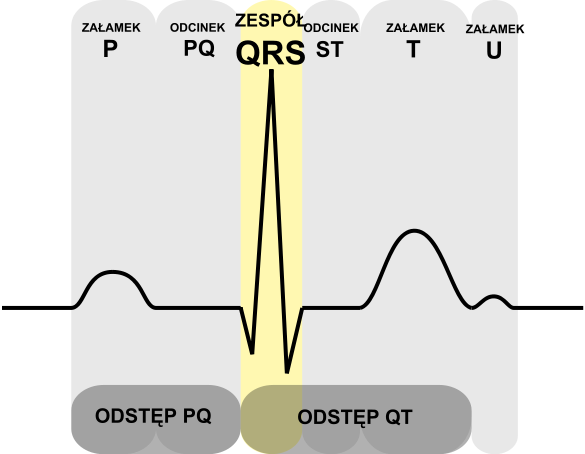
\includegraphics[width=0.8\textwidth]{Grafika/ZespolQRS}
	\caption{Wyidealizowany schemat zapisu EKG z zaznaczonym zespołem QRS. Źródło  \cite{QRSComplexWiki}}
	\label{fig:QRSComplex}
\end{figure}


\qquad Klasyfikacja zespołu QRS ma na celu wyodrębnienie grup zespolów podobnych (w zadanym zakresie tolerancji). Odmienny kształt zespołu jest konsekwencją odmiennie przebiegającego pobudzenia. Klasyfikacja polega na stwierdzeniu przynależności klasyfikowanego zespołu do jednej z istniejących klas albo tworzeni nowych klas, jeżeli przynależności nie stwierdzono \cite{Augustyniak}.

\qquad Celem opisywanego modułu jest wyliczenie liczby klas zespołów QRS, określenie reprezentantów każdej z nich oraz oznaczenie klas zespołów QRS na wykresie ECG. Wyodrębnienie klas QRS występujących w sygnale ECG pozwala na określenie prawidłowości rytmu pracy serca. Z reguły nieregularności mają charakter przejściowy, dlatego ich poprawne wyznaczenie wymaga przeprowadzenia 24-godzinnego badania pracy serca, czyli testu Holtera \cite{RaportKoncowy}.

\qquad W literaturze można spotkać się z różnymi podejściami do klasyfikacji zespołów QRS. W \cite{SVMBasedArrhythmiaClassification} autorzy zaproponowali algorytm polegający na wykorzystaniu liniowej analizy dyskryminacyjnej (LDA) w celu zredukowania wymiaru przestrzeni cech. Do klasyfikacji zastosowano maszynę wektorów nośnych (SVM). Ponadto w pracy tej podjęto próbę klasyfiacji przy pomocy MLP (ang. Multilayer Perceptrons) oraz klasyfikatora FIS (ang. Fuzzy Inference System). Najlepsze rezultaty autorzy otrzymali wykorzystując SVM. Podobne podejście zastosowano w \cite{Abhishek}, gdzie dodatkowo w celu ograniczenia zakłóceń oraz ekstrakcji cech wykorzystano transformację falkową. 
W \cite{Laguna} autorzy stworzyli adaptacyjny algorytm, działający w czasie rzeczywistym, klasyfikujący zespoły QRS. Zaproponowane rozwiązanie bazuje na modelu funkcji Hermite'a. 
W innej pracy autorzy wyekstrahowali cztery konkretne cechy z sygnału ECG, aby następnie wykorzystać odległość Mahalanobisa jako kryterium klasyfikacji \cite{Moreas}.

\qquad Rozwiązanie przyjęte w niniejszej pracy opiera się o ekstrakcję cech z sygnału ECG, klasteryzacji otrzymanych wektorów przy pomocy algorytmu g-means oraz klasyfikacji z wykorzystaniem maszyny wektorów nośnych. Podejście takie podyktowane jest ... / wynika z ... ? TODO: NAPISAC JAKOS ZE WYKORZYSTUJEMY TO CO NAPISALI ROK TEMU


DO ZROBIENIA WE WSTĘPIE:
\begin{enumerate}
	\item cel (jest) i założenia projektu
	\item badania literaturowe - istniejące rozwiązania (vide linki, które wysłałem) 
	\item skróconą koncepcję rozwiązania (ekstrakcja - klasteryzacja - klasyfikacja)
\end{enumerate}

\section{Koncepcja proponowanego rozwiązania}

\quad Algorytm klasyfikacji załamków QRS został podzielony na trzy części. Najpierw dane wejściowe zostają znormalizowane i skwantyzowane, następnie przeprowadzana jest procedura ekstrakcji cech. W drugiej części następuje klasteryzacja wektorów cech zespołów QRS. Polega to na grupowaniu tych danych w klasy, które mają najwięcej wspólnego - leżą najbliżej siebie w przestrzeni o wymiarze równym liczbie porównywanych cech (stosowana jest tutaj metryka Euklidesowa). Warto zaznaczyć, iż każdy współczynnik reprezentuje inną wielkość i z tego powodu wartość tolerancji jest dobierana dla każdego z nich indywidualnie. Do klasteryzacji wykorzystywany jest algorytm G-średnich (ang. "G-means"). W ostatnim kroku następuje klasyfikacja, czyli przyporządkowanie każdego zespołu QRS do jednej z klas. W tym celu wykorzystywana jest metoda wektorów nośnych (ang. "Support Vector Machine", w skrócie SVM).

Dobór tych metod - w tym również wybór klasyfikacji na podstawie wektorów cech, a nie sygnałów - został dokonany przez poprzedni zespół projektowy, a zadaniem autorów niniejszego raportu było przeprowadzenie porównania funkcjonowania tych metod w trzech innych językach programowania niż oryginalny język implementacji.

\subsection{Ekstrakcja cech}
\qquad Zadaniem tej części zastosowanego algorytmu jest wyliczenie pewnych istotnych wskaźników charakteryzujących zespół QRS na podstawie znormalizowanych danych wejściowych. Bazując na implementacji poprzedniego zespołu projektowego, stosowane są współczynniki wymienione poniżej \cite{RaportKoncowy}.
\begin{enumerate}
	\item Początek i koniec całego zespołu QRS,
	\item Wartość szczytowa załamka R,
	\item Interwał między poprzednim a rozważanym załamkiem R,
	\item Interwał między rozważanym a kolejnym załamkiem R,
	\item Wartość szczytowa oraz koniec załamka T,
	\item Początek, wartość szczytowa i koniec załamka P.
\end{enumerate}
Wszystkie te współczynniki powinny być zapisywane po synchronizacji wszystkich wykrytych zespołów, na przykład względem pozycji załamka R \cite{Augustyniak}.

\subsection{Klasteryzacja}
\quad Jak już zostało wspomniane, do grupowania danych w klastry (klasy) użyto algorytmu G-średnich. Jest rozszerzeniem popularnej metody k-średnich, która polega na dobraniu $k$ klas w~zbiorze danych tak, aby każdy punkt należał do klasy, do której środka ciężkości ma najbliżej \cite{KMeans}.

Przyjęto, że dane, które należy pogrupować to $d$-wymiarowe wektory należące do zbioru $X$ o liczności $n$. $S$ to zbiór klas, a więc $S_{j} = \{x_{i} \in X | klasa(x_{i}) = j\}$ dla $i = 1, 2, ..., n$. Zbiór środków ciężkości klas oznaczony został literą $C$ i zdefiniowany jako: $C = \{c_{j} = \frac{\sum_{x \in S_{j}} x}{|S_{j}|}\}$ dla $j = 1, 2, ..., k$.
Cel algorytmu k-średnich to minimalizacja wyrażenia przedstawionego wzorem \ref{eq:kmeans} .
\begin{equation}
\label{eq:kmeans}
\sum_{j=1}^{k}\sum_{x \in S_{j}} \|x - c_{j}\|
\end{equation}

Poważnym problemem tego algorytmu jest fakt, iż liczba klas musi być znana bądź przyjęta z góry, co oznacza posiadanie pewnej wcześniejszej wiedzy na temat klasteryzowanego zbioru danych \cite{GMeans, GMeansExplanation}. W przypadku braku takich informacji, należy zastosować uogólnienie algorytmu k-średnich, które pozwoli dobrać optymalne $k$ względem pewnego wskaźnika jakości.
Algorytm, który został zastosowany w opisywanym module dobiera $k$ tak, aby w każdej klasie rozkład punktów był możliwie bliski rozkładu normalnego. Stąd też wzięła się litera "G" w nazwie - od rozkładu Gaussa \cite{GMeans}.

Metoda G-średnich zaczyna od niewielkiej liczby klas, by później odpowiednio zwiększać $k$ - nie jest przewidziana procedura zmniejszania tego parametru. W pierwszym kroku zwykle przyjmowane jest $k = 1$, z czego wynika, że $C$ jest zbiorem jednoelementowym, zawierającym środek ciężkości całego zbioru $X$ \cite{GMeans}. W każdym kroku algorytm sprawdza, czy dana klasa ma rozkład normalny, a jeśli nie, to dodaje jej dodatkowy środek. Między każdym takim dodawaniem środków jest używana procedura k-średnich, aby poprawić jakość rozwiązania.

Sprawdzenie normalności rozkładu wewnątrz klasy odbywa się za pomocą testu Andersona - Darlinga. Pozwala on rozstrzygnąć, czy znormalizowane dane są rozłożone zgodnie z pewnym rozkładem prawdopodobieństwa. Elementy zbioru danych oznaczono przez $y_{i}, i = 1, 2, ..., n$. Wartość statystyki Andersona - Darlinga oblicza się na podstawie wzoru \ref{eq:a-d}.
\begin{equation}
\label{eq:a-d}
	A^{2} = -n - \frac{1}{n} \sum_{i=1}^{n}(2i - 1)(log(\Phi(y_{i})) + log(1 - \Phi(y_{n-i+1})))
\end{equation}

Gdy wartość średnia i odchylenie standardowe w testowanym zbiorze danych są obliczane na jego podstawie (a nie znane), wartość statystyki należy poprawić według wzoru \ref{eq:a-d-correction} \cite{GMeans}.
\begin{equation}
\label{eq:a-d-correction}
	A^{2*} = A^{2}(1 + \frac{4}{n} + \frac{25}{n^{2}})
\end{equation}

Parametrem wejściowym dla tego testu jest poziom ufności $\alpha$. Jest on zwykle wyrażony w~procentach, bądź w ułamku dziesiętnym. Zależy od niego tzw. wartość krytyczna, czyli próg wartości statystyki, ponad którym odrzucana jest hipoteza o rozkładzie normalnym danych. Wzorem autorów algorytmu G-średnich, użyto $\alpha=0.0001$ \cite{GMeans}.

Test Andersona - Darlinga można stosować tylko do jednowymiarowych danych, a więc należy sprowadzić wyjściowy zbiór (o wymiarze $d$) do przestrzeni liczb rzeczywistych. W tym celu algorytm G-średnich dla każdej klasy używa metody k-średnich z $k=2$ oraz dwoma środkami $c^{1,2}_j = c_j \pm m$, gdzie $m$ jest wektorem o normie niewielkiej w porównaniu z odległościami między punktami w klasie. Niech otrzymane w wyniku tej operacji środki to $c^1$ oraz $c^2$, a wektor $u$ opisuje odległość między nimi: $u = c^1 - c^2$. Cała klasa $S_j$ jest rzutowana prostopadle na wektor $u$, w~wyniku czego otrzymuje się jednowymiarową przestrzeń $S_j '$, dla której po normalizacji stosuje się test Andersona - Darlinga. W przypadku gdy wartość statystki jest mniejsza niż wartość krytyczna dla danej ufności, nowe środki są odrzucane. W przeciwnym razie zachowuje się je, dzieląc klasę $S_j$ na dwie.

Rysunek \ref{fig:g-means-projection} przedstawia przykład takiego rzutowania. Widać na nim dwa nowe środki znalezione przez metodę k-średnich dla danej klasy oraz rzutowanie prostopadłe punktów tej klasy na prostą wyznaczaną przez wektor między tymi dwoma środkami. Jak można się spodziewać, rozkład takiego zbioru danych jest bimodalny, a nie normalny, tak więc te dwa widoczne na rysunku środki zostaną przyjęte.

\begin{figure}
\centering
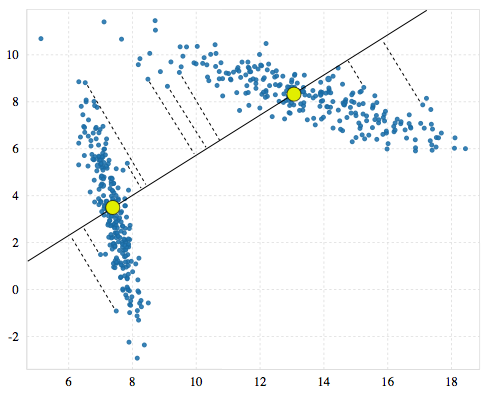
\includegraphics[width=0.7\linewidth]{Grafika/g-means-projection}
\caption{Przykład rzutowania zbioru danych na wektor łączący znalezione środki ciężkości. Źródło: \cite{GMeansExplanation}}
\label{fig:g-means-projection}
\end{figure}

Cały zastosowany algorytm klasteryzacji może być przedstawiony w następujących krokach:
\begin{enumerate}
	\item Jako parametry wejściowe przyjmij zbiór danych oraz ufność testu Andersona-Darlinga.
	\item Wylicz początkowy środek ciężkości: $C = \{\bar{x}\}$.
	\item Wykonaj klasteryzację: C = k-średnich(X, C).
	\item Dla każdej klasy $S_j$ sprawdź jej rozkład testem Andersona-Darlinga:
	\begin{enumerate}
		\item Wylicz dwa środki pochodne $c_j^1, c_j^2$.
		\item Wykonaj ponowną klasteryzację: $\{c^1, c^2\} = k-"srednich(S_j, \{c_j^1, c_j^2\})$.
		\item Wyznacz wektor $u = c^1 - c^2$.
		\item Wyznacz jednowymiarową przestrzeń $S_j '$.
		\item Wylicz wartość statystyki Andersona - Darlinga dla $S_j '$.
		\item Jeśli jest ona większa od wartości krytycznej, podziel klasę $S_j$ na dwie ze środkami $c^1$ oraz $c^2$. Jeśli jest mniejsza, zachowaj poprzedni środek.
	\end{enumerate}
	\item Powtarzaj od kroku 3 dopóki żadne nowe środki nie zostaną dodane.
\end{enumerate}

\subsection{Klasyfikacja}
\quad Aby sklasyfikować powstałe w poprzednim kroku klastry wykorzystano klasyfikator SVM (Support Vector Machine). Problem klasyfikacji wymaga podziału zbioru danych wejściowych na zbiór uczący oraz zbiór testowy. Każdy z elementów zbioru uczącego zawiera wartość oczekiwaną (np. etykieta klasy) oraz jakąś ilość atrybutów (np. wektor cech). Celem SVM jest stworzenie modelu (bazujcego na danych uczących), który przewiduje nieznaną wartość oczekiwaną (etykietę) dla podanego na wejściu elementu zbioru testowego. 

W najprostszej postaci klasyfikator SVM służy do wyznaczenia hiperpłaszczyzny rozdzielającej dwa liniowo separowalne zbiory. Hiperpłaszczyzna ta wyznaczana jest z maksymalnym marginesem, tzn. tak, aby suma jej odległości od najbliższych próbek z obu klas była jak największa (patrz rys. \ref{fig:SVM}).

\begin{figure}[h]
	\centering
	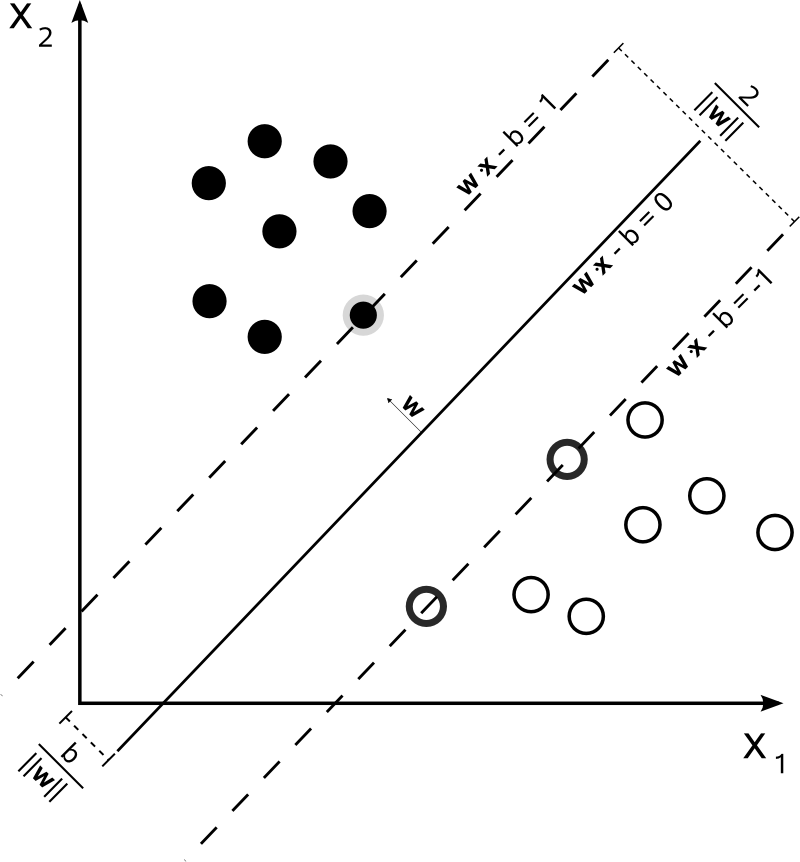
\includegraphics[width=8cm]{Grafika/Svm_max_sep_hyperplane_with_margin}
	\caption{Dwuwymiarowy przypadek hiperpłaszczyzny rozdzielającej dwie klasy z zaznaczonym marginesem. Źródło \cite{SVMWiki}}
	\label{fig:SVM}
\end{figure}

Mając dany zbiór uczący, będący zbirem par składających się z wektora cech oraz etykiety $(x_i, y_i)$, $i = 1,...,l$, gdzie $x_i \in \mathbb{R}^n$ i $y_i \in \{1,-1\}$, maszyna wektorów nośnych (SVM) wymaga rozwiązania następującego problemu optymalizacji \cite{csie}:

\begin{equation}
\label{eq:SVMOptProb}
\min\limits_{w,b,\xi} \frac{1}{2}w^Tw+C\sum_{i=1}^{l}\xi_i
\end{equation}

z ograniczeniem:

\begin{equation}
\label{eq:SVMOptProbCond}
\begin{array}{l}
y_i\left(w^T\phi\left(x_i\right)+b\right) \geqslant 1-\xi_i,\\
\xi_i > 0
\end{array}
\end{equation}


W wielu przypadkach nie można zagwarantować liniowej separowalności zbiorów.  W takich sytuacjach stosuje się tzw. Kernel Trick. Polega to na zwiększeniu wymiaru przestrzeni danych wejściowych, aby w nowej przestrzeni istniała własność liniowej separowalności zbiorów.

W zdefiniowanym wzorami (\ref{eq:SVMOptProb}) oraz (\ref{eq:SVMOptProbCond}) problemie optymalizacji wektor uczacy $x_i$ przekształcany jest do przestrzeni o większym wymiarze dzięki funkcji $\phi$. Parametr $C>0$ jest karą za niespełnienie warunków zadania. Ponadto, funkcja $K(x_i,x_j)=\phi(x_i)^T\phi(x_j)$ jest nazywana funkcją jądra (ang. kernel function). Poniżej wypisano cztery przykładowe funkcje jądra, jakie można spotkać w literaturze poświęconej SVM.

\begin{enumerate}
	\item Liniowa: $K\left(x_i,y_j\right)=x_i^Tx_j$
	\item Wielomianowa: $K\left(x_i,y_j\right)=\left(\gamma x_i^Tx^j+r\right)^d, \gamma > 0$
	\item Radialna funkcja bazwa (RBF): $K\left(x_i,y_j\right)=\exp{\left(-\gamma \|x_i-x_j\|^2\right)}, \gamma > 0$
	\item Sigmoida: $K\left(x_i,y_j\right)=\tanh{\left(\gamma x_i^Tx_j+r\right)}$
\end{enumerate}

W opisywanym module wykorzystana została funkcja RBF (ang. Radial Basis Function).

Aby klasyfikator mógł działać wcześniej należy go wytrenować. Polega to na podaniu mu ciągu wektorów uczących. Opisywany klasyfikator został wytrenowany za pomocą bazy danych MIT-BIH Arrhythmia Database \cite{MITDB}. Gotowy model klasyfikatora wczytywany jest z pliku, w którym zapisane są różne parametry oraz zestaw wektorów nośnych, na których opiera się działanie metody SVM.


\section{Rezultaty i wnioski}

\subsection{Funkcjonowanie algorytmu G-średnich}

\begin{table}[!tp]
	\centering
	\caption{Liczby klas wyliczonych przez G-means}
	\label{tabResults2}
	\begin{tabular}{|c|c|c|c|}
		\hline
		Nr paczki z MIT-BIH & Matlab & Python & Julia\\ \hline		
		100 & 16 & 16 & 16\\ \hline
		101 & 14 & 16 & 16\\ \hline
		102 & 14 & 16 & 16\\ \hline
		103 & 27 & 16 & 16\\ \hline
		104 & 29 & 16 & 16\\ \hline
		105 &  1 & 20 & 20\\ \hline
		106 & 35 & 16 & 16\\ \hline
		107 & 31 & 16 & 16\\ \hline
		108 & 32 & 15 & 15\\ \hline
		109 &  1 & 21 & 21\\ \hline
		111 & 22 & 17 & 17\\ \hline
		112 & 15 & 19 & 19\\ \hline
		113 & 13 & 16 & 16\\ \hline
		114 &  1 & 15 & 15\\ \hline
		115 & 15 & 16 & 16\\ \hline
		116 &  1 & 16 & 16\\ \hline
		117 & 23 & 16 & 16\\ \hline
		119 & 33 & 16 & 16\\ \hline
		121 & 27 & 16 & 16\\ \hline
		122 & 29 & 21 & 21\\ \hline
		123 &  1 & 16 & 16\\ \hline
		124 & 30 & 15 & 15\\ \hline
		200 & 32 & 20 & 20\\ \hline
		201 & 56 & 13 & 13\\ \hline
		202 & 29 & 21 & 21\\ \hline
		203 &  1 & 26 & 26\\ \hline
		205 &  1 & 21 & 21\\ \hline
		208 & 36 & 24 & 24\\ \hline
		209 & 21 & 31 & 31\\ \hline
		210 &  1 & 20 & 20\\ \hline
		212 & 18 & 25 & 25\\ \hline
		213 & 28 & 32 & 32\\ \hline
		214 & 33 & 18 & 18\\ \hline
		215 & 18 & 32 & 32\\ \hline
		217 & 65 & 17 & 17\\ \hline
		219 & 36 & 15 & 15\\ \hline
		220 & 22 & 16 & 16\\ \hline	
		221 & 33 & 19 & 19\\ \hline
		222 &  1 & 22 & 22\\ \hline
		223 &  1 & 18 & 18\\ \hline
		230 & 15 & 20 & 20\\ \hline
		231 & 39 & 12 & 12\\ \hline
		232 & 28 & 17 & 17\\ \hline
		233 & 42 & 24 & 24\\ \hline
		234 & 27 & 29 & 29\\ \hline
	\end{tabular}
\end{table}


\subsection{Funkcjonowanie algorytmu SVM}

\begin{figure}[!htp]
	\centering
	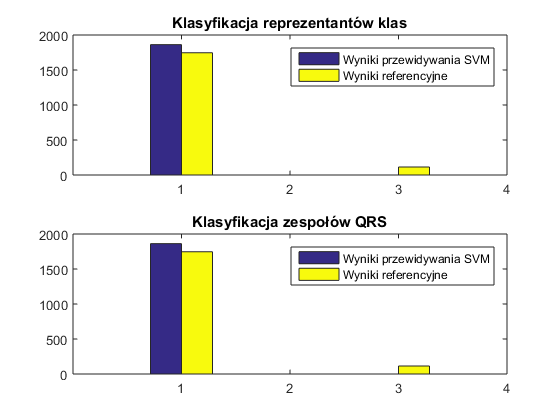
\includegraphics[width=15cm]{Grafika/101_2_3}
	\caption{Histogramy klasyfikacji zespołów dla paczki danych o numerze 101}
	\label{fig:hist1}
\end{figure}

W przypadku implementacji w Matlabie wykorzystano bibliotekę libsvm \cite{csie}. Istnieje również wersja tej biblioteki przeznaczona do wykorzystania w Pythonie, jednak po licznych, nieudanych próbach wykorzystania jej zdecydowano się zaimplementować własną maszynę wektorów nośnych w oparciu o pliki źródłowe biblioteki libsvm. Analogicznie postąpiono w przypadku implementacji w Julii. Efektem tego jest krótszy czas wykonywania się modułu napisanego w Matlabia (patrz Tab.\ref{tabResults}), a wynika to między innymi z braku doświadczenia związanego z optymalizacją kodu w wykorzystanych językach programowania.

\begin{table}[!tp]
	\centering
	\caption{Czasy wykonywania programu w poszczególnych językach dla różnych paczek danych. Wyniki wyrażone w sekundach}
	\label{tabResults}
	\begin{tabular}{|c|c|c|c|c|}
		\hline
		Nr paczki z MIT-BIH & C++ & Matlab & Python & Julia\\ \hline		
		
		100 & 2.7842 & 1.9523 & 12.8154 & 5.9019\\ \hline
		101 & 2.4618 & 1.4195 & 10.4921 & 1.8999\\ \hline
		102 & 2.7384 & 1.2609 & 12.2422 & 2.2158\\ \hline
		103 & 3.2374 & 2.3951 & 11.7082 & 2.1800\\ \hline
		104 & 2.6769 & 1.6457 & 11.8960 & 2.1335\\ \hline
		105 & 3.4991 & 1.3186 & 14.7023 & 3.1231\\ \hline
		106 & 2.3171 & 1.8217 & 10.3660 & 2.1149\\ \hline
		107 & 2.2940 & 1.5331 &  9.9881 & 2.0690\\ \hline
		108 & 1.9152 & 1.7391 &  8.5037 & 2.1076\\ \hline
		109 & 3.2367 & 1.2506 & 13.9100 & 3.4216\\ \hline
		111 & 2.6589 & 1.8369 & 11.5751 & 2.8741\\ \hline
		112 & 3.2395 & 2.2931 & 14.7076 & 3.3450\\ \hline
		113 & 2.3822 & 1.2857 & 10.2796 & 1.9384\\ \hline
		114 & 1.2847 & 0.5056 &  5.5476 & 1.5342\\ \hline
		115 & 2.7577 & 1.2325 & 11.0596 & 2.2074\\ \hline
		116 & 3.6987 & 1.242  & 13.3443 & 2.5876\\ \hline
		117 & 2.1506 & 1.506  &  8.4621 & 1.6437\\ \hline
		119 & 8.4046 & 1.5771 & 10.9920 & 2.0713\\ \hline
		121 & 2.4702 & 2.0902 & 10.2799 & 1.9764\\ \hline
		122 & 4.0723 & 2.0928 & 14.2113 & 3.1179\\ \hline
		123 & 2.0768 & 0.7942 &  8.3970 & 1.7214\\ \hline
		124 & 1.9720 & 1.6778 &  8.1376 & 1.7144\\ \hline
		200 & 2.5885 & 1.8849 & 11.5171 & 2.8278\\ \hline
		201 & 2.3562 & 1.8963 &  9.2493 & 1.8646\\ \hline
		202 & 2.7007 & 2.132  & 13.7891 & 3.7784\\ \hline
		203 & 3.1012 & 1.2565 & 14.5795 & 3.1471\\ \hline
		205 & 3.3001 & 1.3475 & 15.0669 & 3.2603\\ \hline
		208 & 4.4140 & 2.4411 & 15.5731 & 3.5292\\ \hline
		209 & 3.9942 & 2.139  & 17.3970 & 4.0028\\ \hline	
		210 & 3.2321 & 1.1721 & 26.9134 & 6.4331\\ \hline
		212 & 3.5982 & 2.9475 & 26.8902 & 3.3901\\ \hline
		213 & 4.1917 & 2.3988 & 31.4794 & 4.1461\\ \hline
		214 & 2.6582 & 1.8288 & 18.5719 & 2.4209\\ \hline
		215 & 4.5147 & 1.6584 & 30.4394 & 3.9549\\ \hline
		217 & 2.5368 & 2.0103 & 18.7012 & 2.5877\\ \hline
		219 & 2.8246 & 1.8043 & 19.7484 & 3.2817\\ \hline
		220 & 2.7018 & 1.2670 & 18.7101 & 2.6660\\ \hline		
		221 & 3.0609 & 1.7631 & 13.7086 & 3.0062\\ \hline
		222 & 3.1459 & 1.2655 & 14.3837 & 3.2238\\ \hline
		223 & 3.0877 & 1.2356 & 13.7317 & 3.0060\\ \hline
		230 & 2.7823 & 1.8286 & 14.1915 & 2.8759\\ \hline
		231 & 2.0888 & 1.4458 &  8.6989 & 3.3912\\ \hline
		232 & 2.2694 & 1.3707 & 10.3214  & 2.355\\ \hline
		233 & 3.4706 & 2.5759 & 15.5837 & 3.4776\\ \hline
		234 & 3.3963 & 3.6223 & 16.4922 & 3.5836\\ \hline
		\textbf{Czas średni} & \textbf{3.029401} & \textbf{1.5836} & \textbf{20.6123} & \textbf{2.3554}\\ \hline
	\end{tabular}
\end{table}

\subsection{Wnioski}

Krótki czas wykonywania programu napisanego w Matlabie wynika głównie z wykorzystania biblioteki libsvm, która jest napisana w C. Dla pozostałych języków zaimplementowano maszynę wektorów nośnych w oparciu o pliki źródłowe wspomnianej biblioteki.

Wykorzystanie metody SVM z szesnastoelementowym wektorem cech wydaje się złym rozwiązaniem, gdyż niemal zawsze wektor klasyfikowany jest do jednej klasy - patrz Rys.\ref{fig:hist1}. Poza zbyt licznym wektorem cech wpływ na to ma również fakt, że około 90\% zespołów QRS z bazy MIT-BIH reprezentują pobudzenia nadkomorowe. Rozwiązaniem problemu klasyfikacji może okazać się odpowiednie zmniejszenie liczności wykorzystywanego wektora cech.

Przeprowadzono również testy, w których SVM korzystał z różnych modeli (wygenerowanych z różnych paczek danych). Zaobserwowano, że normalizacja wektorów uczących znacznie przyspiesza proces uczenia, czego potwierdzeniem jest Rys.\ref{fig:SVM}.

\begin{figure}[!htp]
	\centering
	\includegraphics[width=15cm]{Grafika/SVMTrain}
	\caption{Wpływ normalizacji na czas nauki SVM}
	\label{fig:TrainNormSVM}
\end{figure}



<Coś o gmeans - że w C++ nie było, a tutaj jest>



\section{Podsumowanie}

W ramach projektu zaimplementowano moduł HeartClass w trzech różnych językach programowania: Matlabie, Pythonie (3.4.x) oraz Julii (0.4.x). Moduł ten ma celu klasyfikowanie zespołów QRS sygnału EKG. W pracy udało się zaimplementować moduł odpowiedzialny za klasteryzację oraz klasyfikację. Z wykonanych testów wynika, że moduł najszybciej wykonuje się w Matlabie. Powodem tego jest głównie fakt, iż w tym module wykorzystano gotową bibliotekę, a nie, jak w przypadku pozostałych dwóch, gdzie zaimplementowano własną maszynę SVM. Dużym zaskoczeniem okazała się implementacja w Julii. Moduł średnio wykonuje się prawie 10 razy szybciej niż w Pythonie i nie wiele wolniej niż w Matlabie.



%----------------------------------------------------------------------------------------
%	REFERENCE LIST
%----------------------------------------------------------------------------------------

\bibliographystyle{alpha}
\begin{thebibliography}{99} % Bibliography - this is intentionally simple in this template

%\bibitem[1]{Figueredo:2009dg}
%Figueredo, A.~J. and Wolf, P. S.~A. (2009).
%\newblock Assortative pairing and life history strategy - a cross-cultural
%  study.
%\newblock {\em Human Nature}, 20:317--330.
 
\bibitem{QRSComplexWiki}
QRS Complex,
\newblock \texttt{https://en.wikipedia.org/wiki/QRS\_complex} .
\newblock Stan na: 05.12.2015 r.

\bibitem{RaportKoncowy}
Studenci Automatyki i Robotyki.
\newblock{\em ESDMiT - Raport końcowy}.
\newblock 04.02.2015 r.

\bibitem{KMeans}
MacQueen, J.
\newblock{\em Some methods for classification and analysis of multivariate observations}.
\newblock W materiałach: "Fifth Berkeley Symposium on Mathematical Statistics and Probability, Volume 1: Statistics", strony 281-297,
\newblock University of California Press, Berkeley, Kalifornia, USA, 1967. 

\bibitem{GMeans}
Hamerly G., Elkan Ch.
\newblock{\em{Learning the k in k-means}}.
\newblock W: Neural Information Processing Systems,
\newblock MIT Press, 2003.

\bibitem{GMeansExplanation}
Użytkownik 'ashenfad'.
\newblock{\em Divining the 'K' in K-means Clustering}.
\newblock \texttt{http://blog.bigml.com/2015/02/24/divining-the-k-in-k-means-clustering/}. 
\newblock Dodane: 24.02.2015 r.
\newblock Stan na: 05.12.2015 r.

\bibitem{SVMWiki}
Support vector machine,
\newblock \texttt{https://en.wikipedia.org/wiki/Support\_vector\_machine} .
\newblock Stan na: 05.12.2015 r.

\bibitem{MITDB}
MIT-BIH Arrhythmia Database,
\newblock \texttt{https://www.physionet.org/physiobank/database/mitdb/}
\newblock Stan na: 05.12.2015 r.

\bibitem{SVMBasedArrhythmiaClassification}
Mi Hye Song, Jeon Lee, Sung Pil Cho, Kyoung Joung Lee, and Sun Kook Yoo,
\newblock Support Vector Machine Based Arrhythmia Classification Using Reduced Features,
\newblock 
International Journal of Control, Automation, and Systems, vol. 3, no. 4, pp. 571-579, December 2005 

\bibitem{Abhishek}
Abhishek S. Thakare,
\newblock QRS Complex Detection and Arrhythmia Classification

\bibitem{Laguna}
P. Laguna, R. Jane, P. Caminal,
\newblock Adaptive Feature Extraction for QRS Classification and Ectopic Breat Detection,
\newblock Institut de Cibernetica, Barcelona, Spain


\bibitem{Moreas}
JCTB Moraes, MO Seixas, FN Vilani, EV Costa,
\newblock A Real Time QRS Complex Classification Method using Mahalanobis Distance,
\newblock Escola Politécnica da Universidade de São Paulo, São Paulo, SP, Brazil

\bibitem{Augustyniak}
P. Augustyniak,
\newblock Przetwarzanie Sygnałów Elektrodiagnostycznych,
\newblock Uczelniane Wydawnictwo Naukowo-Dydaktyczne, Kraków 2001

\end{thebibliography}

\renewcommand\appendixpagename{Dodatek} %Troche bez sensu. Nie wiem jak to zrobic inaczej
\begin{appendices}
	\section{Zagadnienia Implementacyjne}

Zasadę działania zaimplementowanego modułu można opisac w trzech następujących krokach:
\begin{itemize}
	\item Ekstrakcja cech
	\item Klasteryzacja
	\item Klasyfikacja
\end{itemize}

Wejściem modułu są wektory danych otrzymywanych z poprzednich modułów. Na etapie ekstrakcji cech wybierane są cechy, z których składać się będą wektory podlegajace klasyfikacji. !!!!!!!!DOPISAĆ ALBO OLAĆ!!!!!!!!!!!!


<Podrozdziały: "Ciekawsze aspekty wykonanych implementacji", "Instrukcja uruchomienia", "Różnice względem kodu w C++>
\end{appendices}

%\end{multicols}

\end{document}
